\subsection{Welcome}
\begin{frame}{Motivation}
\vspace{-10pt}
We expect climate change to increase storm surge hazard~\cite{SROCC} as:\\
\begin{itemize}
\item Hotter surface temperatures increase the intensity of tropical cyclones (TCs),
      as their ability to do work comes from the heat contrast between their
      bottom and top~\cite{emanuel1991theory}.
 \item Sea level rise puts more areas at risk (see e.g.~\cite{kulp2019new}).
 \end{itemize}
\textbf{But by how much, where, and what is the error?}
\begin{figure}
\centering
    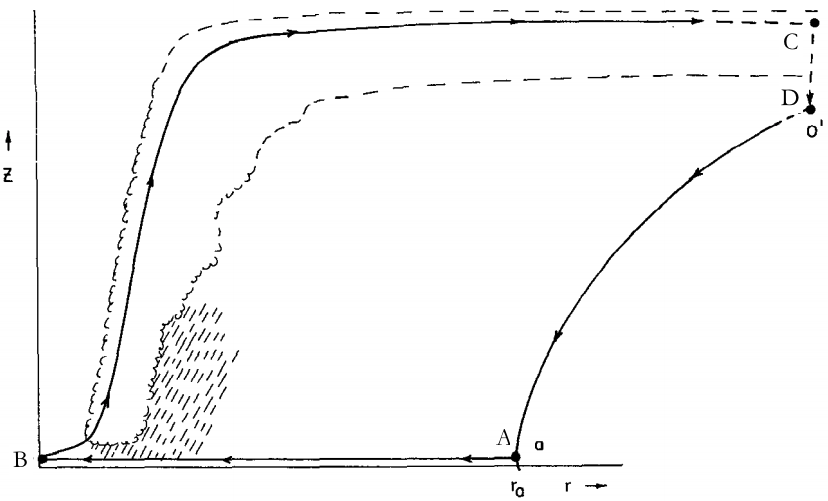
\includegraphics[width=0.49\linewidth]{images/hurricane-carnot.png}\\
    \textit{Figure 1 from~\cite{emanuel1991theory}. }
\end{figure}
\end{frame}

\begin{frame}{Cambridge Flooding Prediction~\cite{kulp2019new, kulp2018coastaldem}}
\vspace{-30pt}
\begin{figure}[htb!]
    \centering
    \hspace{-20pt}
    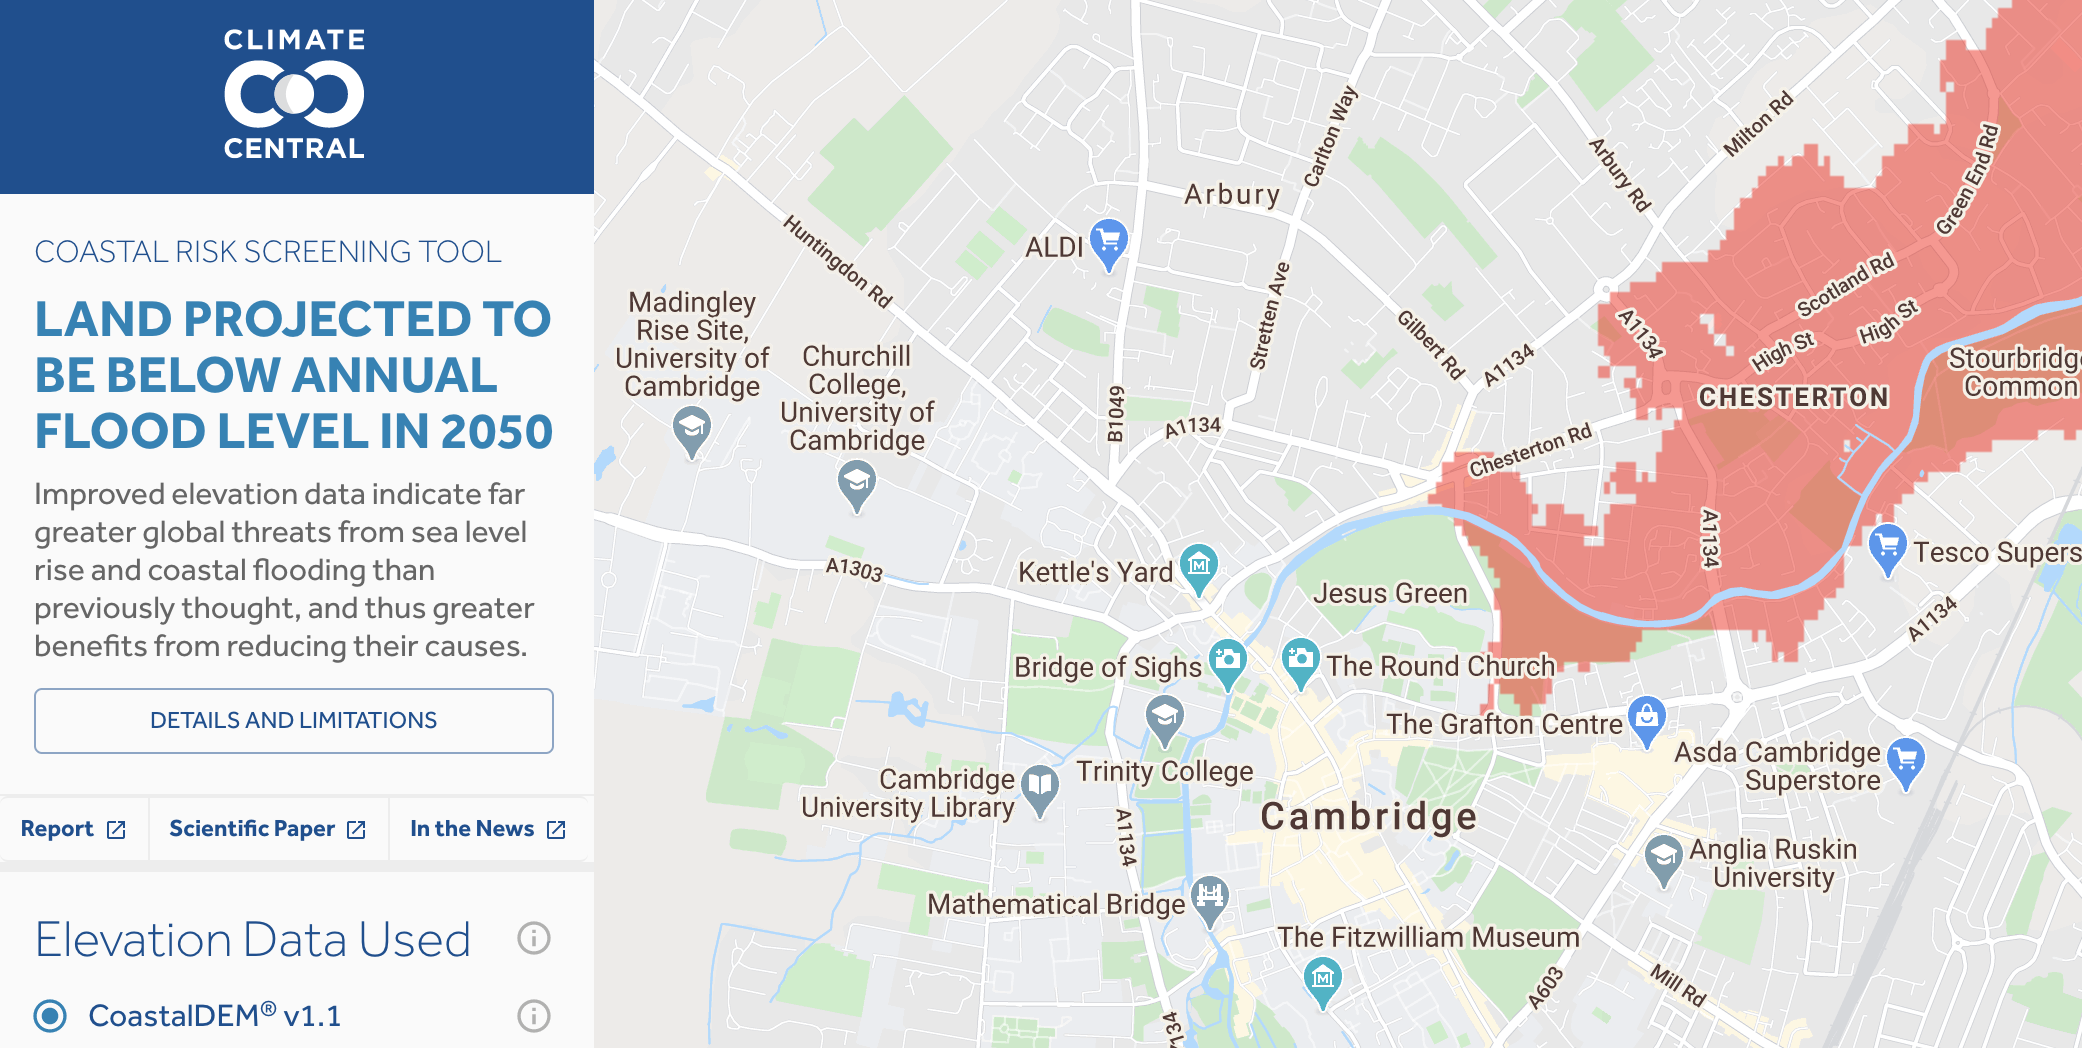
\includegraphics[width=0.9\paperwidth]{images/example-images/cambridge-surge.png}
    \vspace{-7pt}
    \caption{\url{https://coastal.climatecentral.org/map/}}
    \label{fig:}
\end{figure}
\end{frame}

\begin{frame}{New Orleans Flooding Prediction~\cite{kulp2019new, kulp2018coastaldem}}
\vspace{-20pt}
\begin{figure}[htb!]
    \centering
   \hspace{-20pt}
    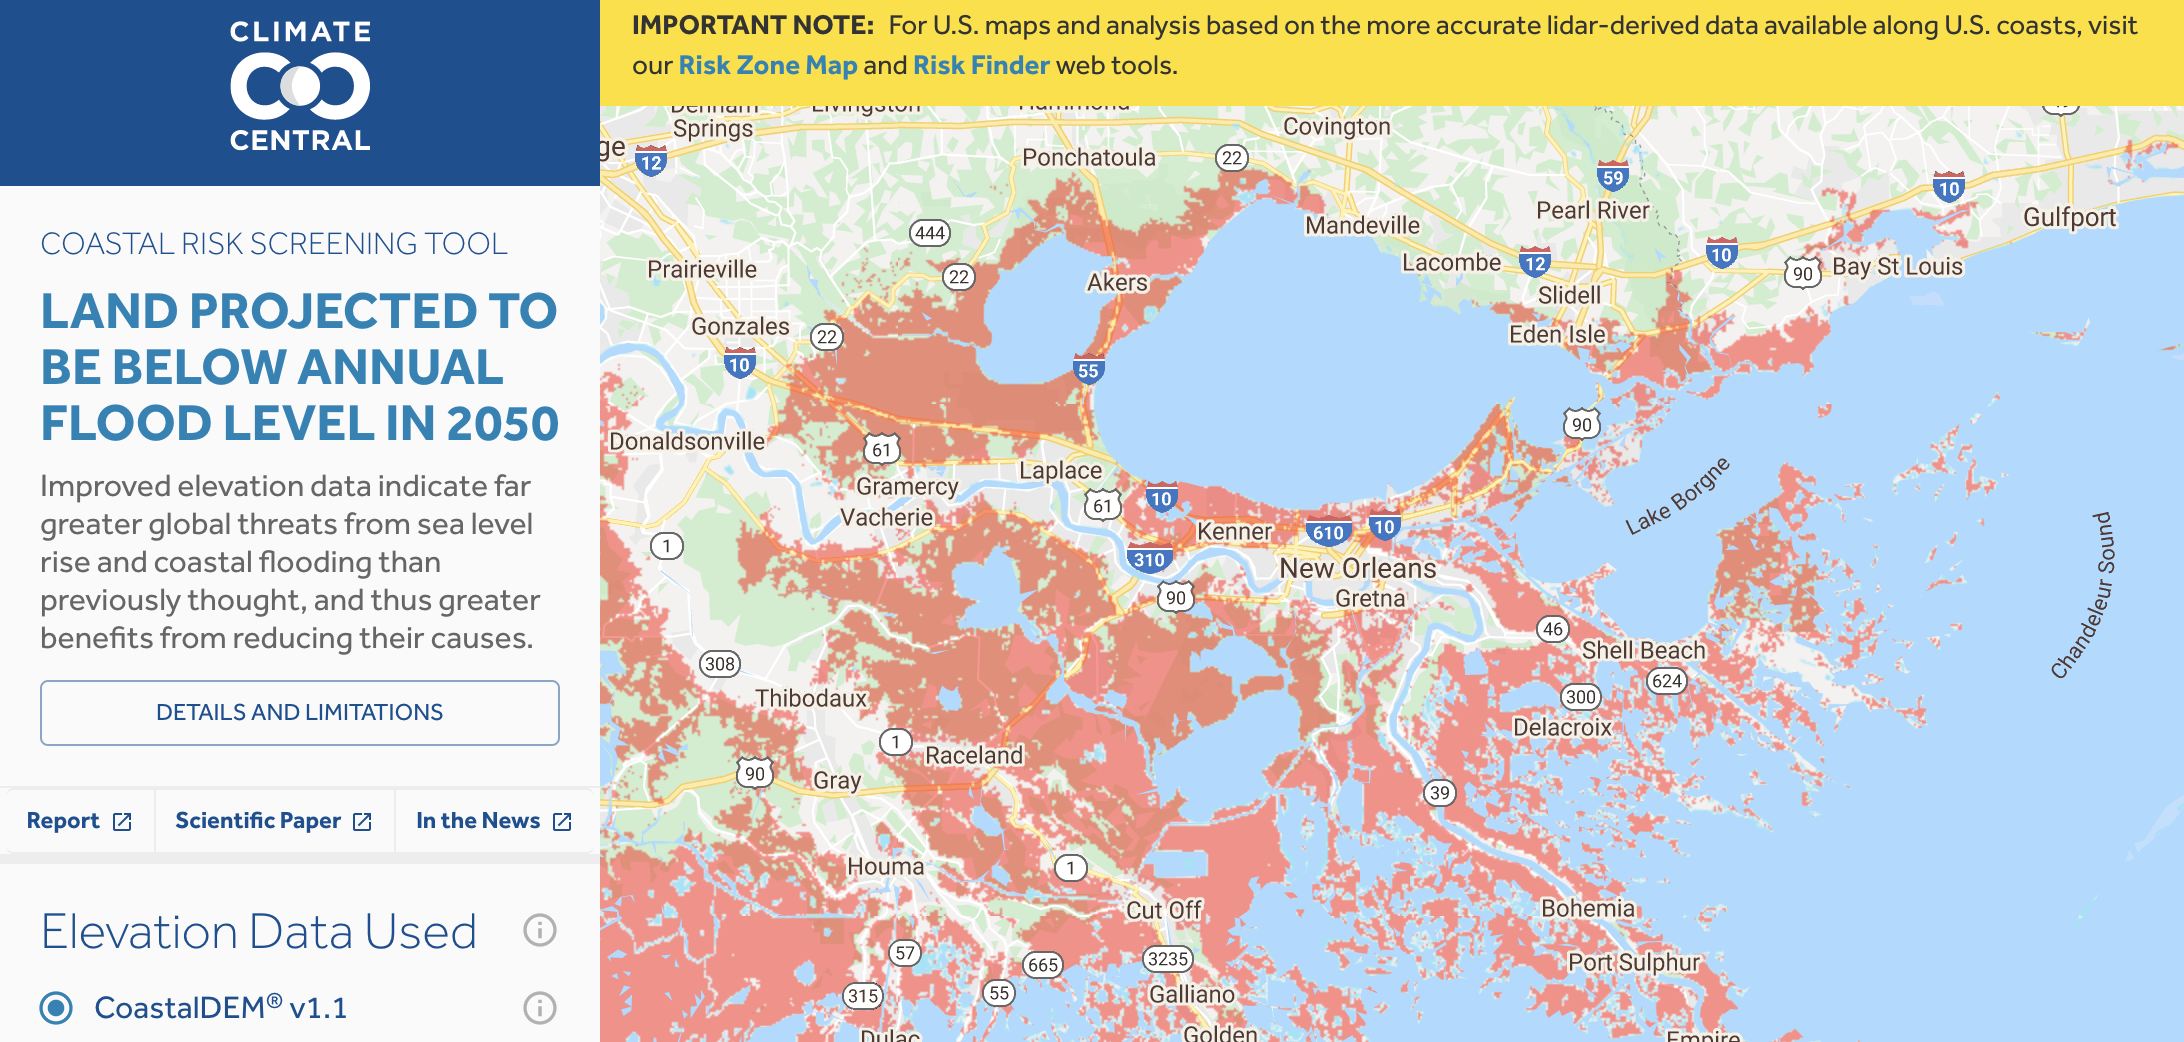
\includegraphics[width=0.9\paperwidth]{images/example-images/new-orleans-surge.png}
    \vspace{-7pt}
    \caption{\url{https://coastal.climatecentral.org/map/}}
    \label{fig:}
\end{figure}
\end{frame}

\begin{frame}{Structure}

This talk covers:
\vspace{5pt}

\begin{enumerate}
    \item A brief introduction to ORCA12 (the model used).
    \item The method of extraction of data from the model.
    \item Computing and justifying local coastal metrics.
     \item Initial local regression results.
\end{enumerate}
\begin{figure}[htb!]
    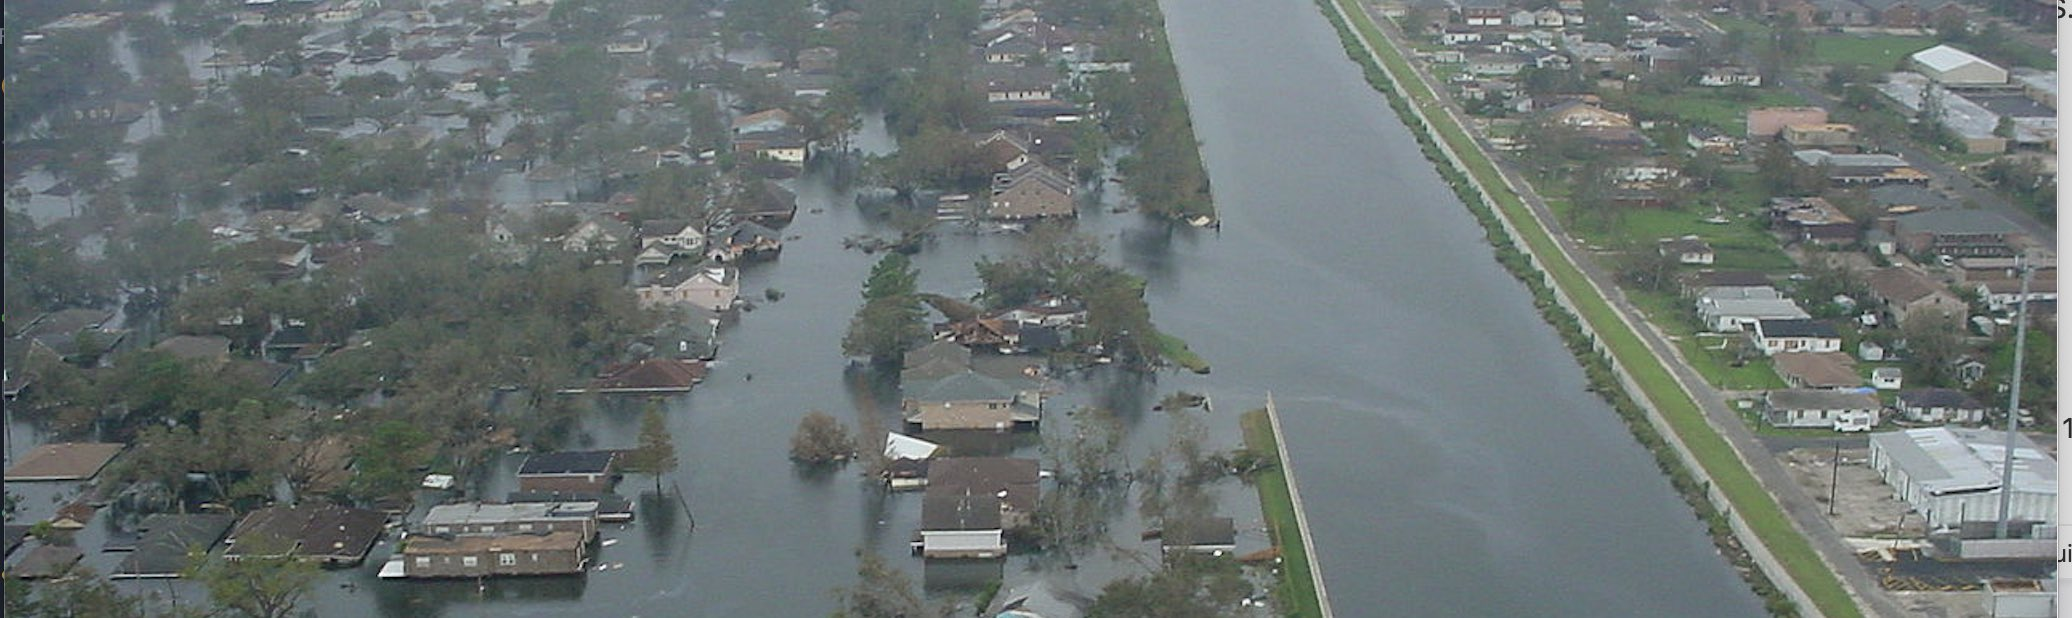
\includegraphics[width=0.9\linewidth]{images/example-images/new-orleans.jpg}
\end{figure}

This work was inspired by Yin et al.~2020~\cite{ZannaPreprint}.\\
Please contact me if you have any suggestions!
\href{mailto:sdat2@cam.ac.uk}{sdat2@cam.ac.uk}
or \href{mailto:sithom@bas.ac.uk}{sithom@bas.ac.uk}.
\begin{center}
\end{center}
\end{frame}
 
